% corrected LN 96
\onecolumn
\newpage
\clearpage
\section{Appendix}
\textbf{Training on English dataset:}

% train on 13311 samples and testing on 4438 samples

% \begin{enumerate}[label=\arabic*.]
%   \item Feedforward:
    \begin{figure}[H]
      \centering
      \subfloat[Feedforward's accuracy using SGD.]{{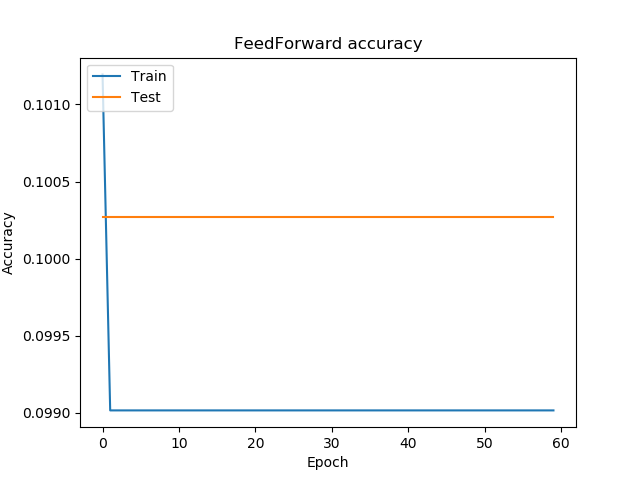
\includegraphics[scale=0.5]{sgdffa.png} }}%
      \qquad
      \subfloat[Feedforward's accuracy using Adam.]{{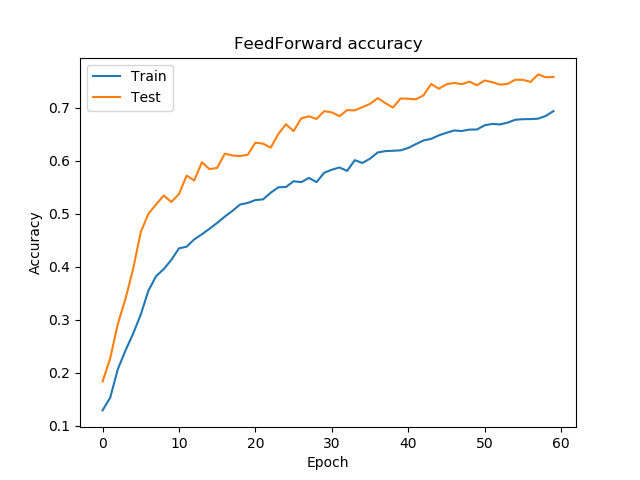
\includegraphics[scale=0.5]{adamffa.png} }}%
      \caption{Accuracy comparison between feedforward using SGD and Adam.}%
      \label{ffa}
    \end{figure}
    \begin{figure}[H]
      \centering
      \subfloat[Feedforward's loss using SGD.]{{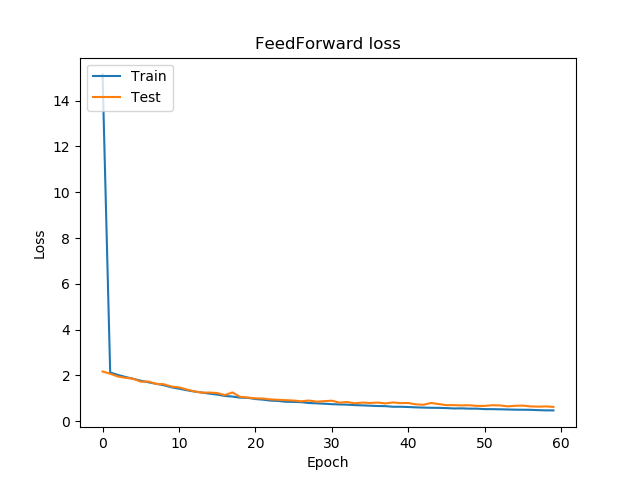
\includegraphics[scale=0.5]{sgdffl.png} }}%
      \qquad
      \subfloat[Feedforward's loss using Adam.]{{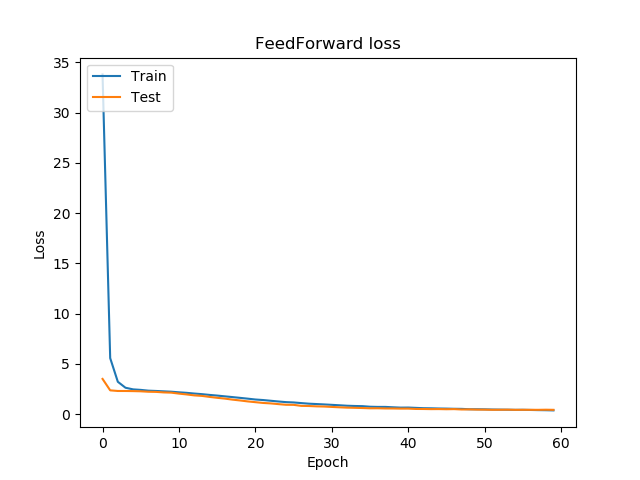
\includegraphics[scale=0.5]{adamffl.png} }}%
      \caption{Loss comparison between feedforward using SGD and Adam.}%
      \label{ffl}
    \end{figure}
  % \item RNN:
    \begin{figure}[H]
      \centering
      \subfloat[RNN's accuracy using SGD.]{{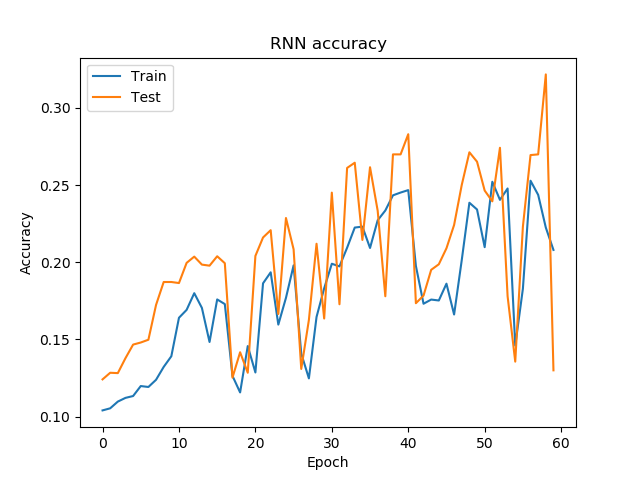
\includegraphics[scale=0.5]{sgdrnna.png} }}%
      \qquad
      \subfloat[RNN's accuracy using Adam.]{{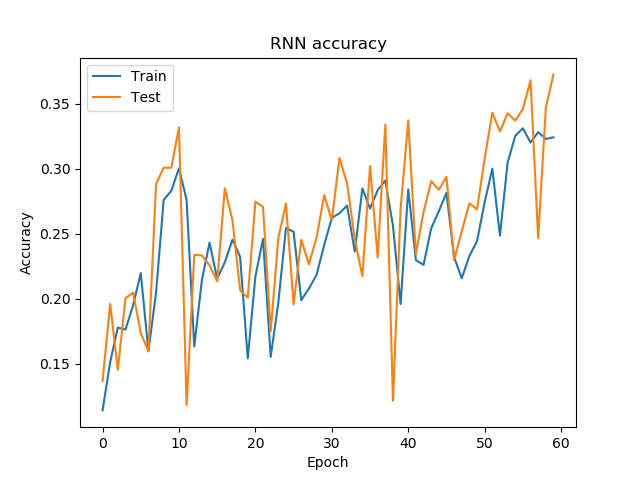
\includegraphics[scale=0.5]{adamrnna.png} }}%
      \caption{Accuracy comparison between RNN using SGD and Adam.}%
      \label{rnna}
    \end{figure}
    \begin{figure}[h]
      \centering
      \subfloat[RNN's loss using SGD.]{{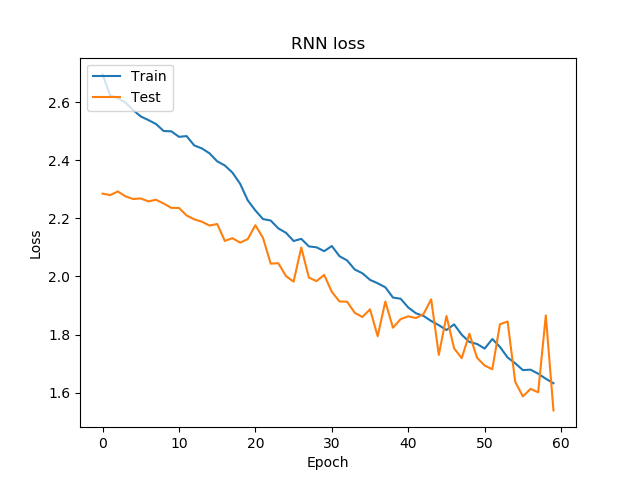
\includegraphics[scale=0.5]{sgdrnnl.png} }}%
      \qquad
      \subfloat[RNN's loss using Adam.]{{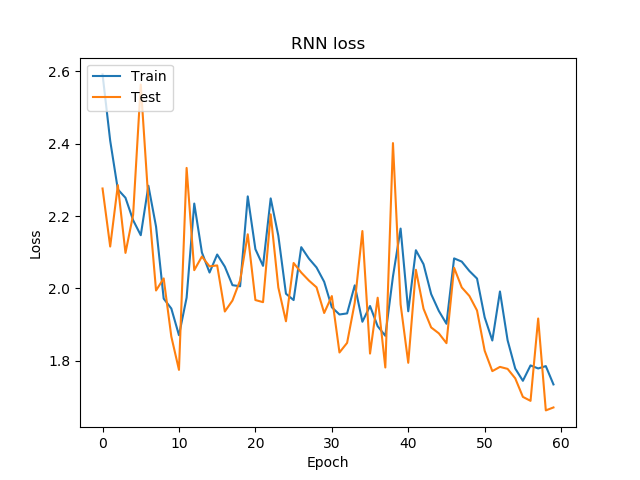
\includegraphics[scale=0.5]{adamrnnl.png} }}%
      \caption{Loss comparison between RNN using SGD and Adam.}%
      \label{rnnl}
    \end{figure}
    \begin{figure}[h]
      \centering
      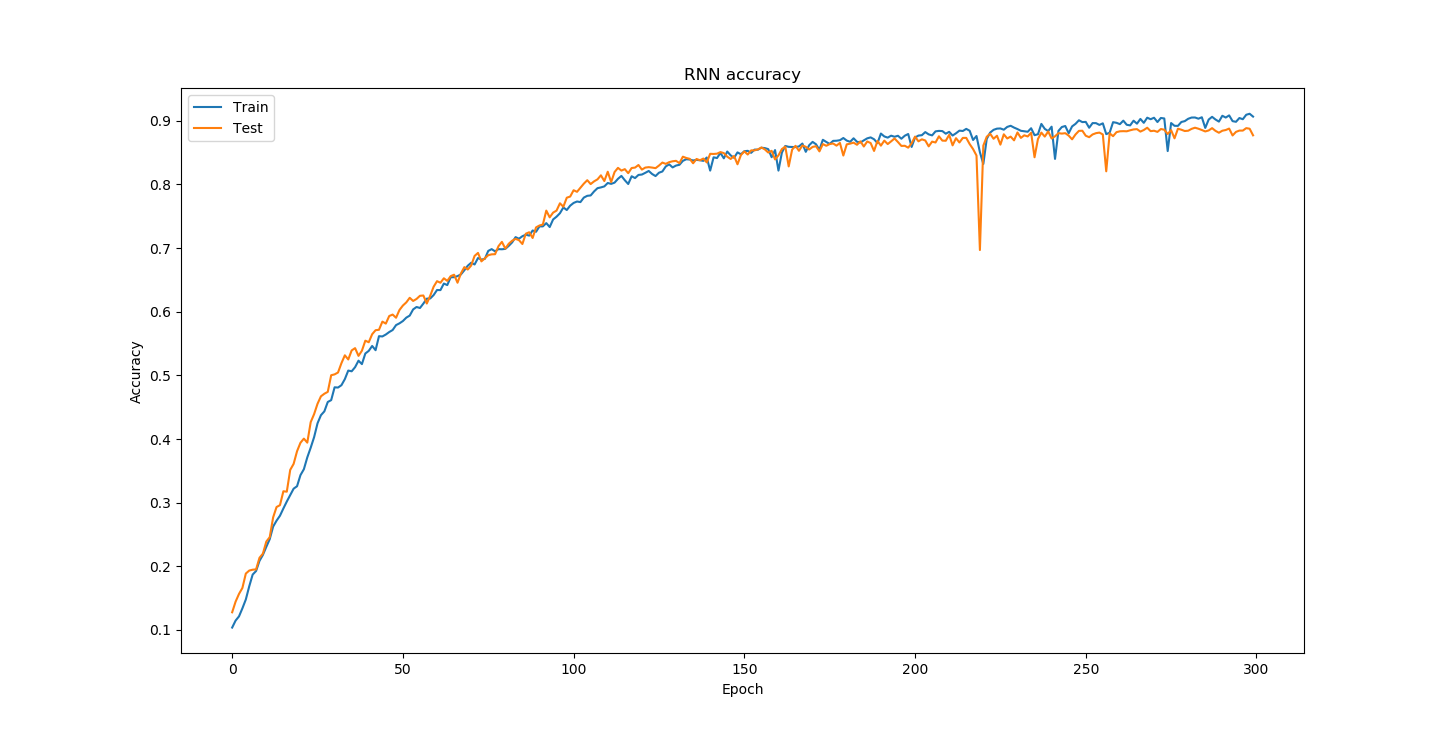
\includegraphics[scale=0.4]{300rnna.png}
      \caption{Training and validation accuracy of RNN model.}
      \label{300rnna}
    \end{figure}

    \begin{figure}[h]
      \centering
      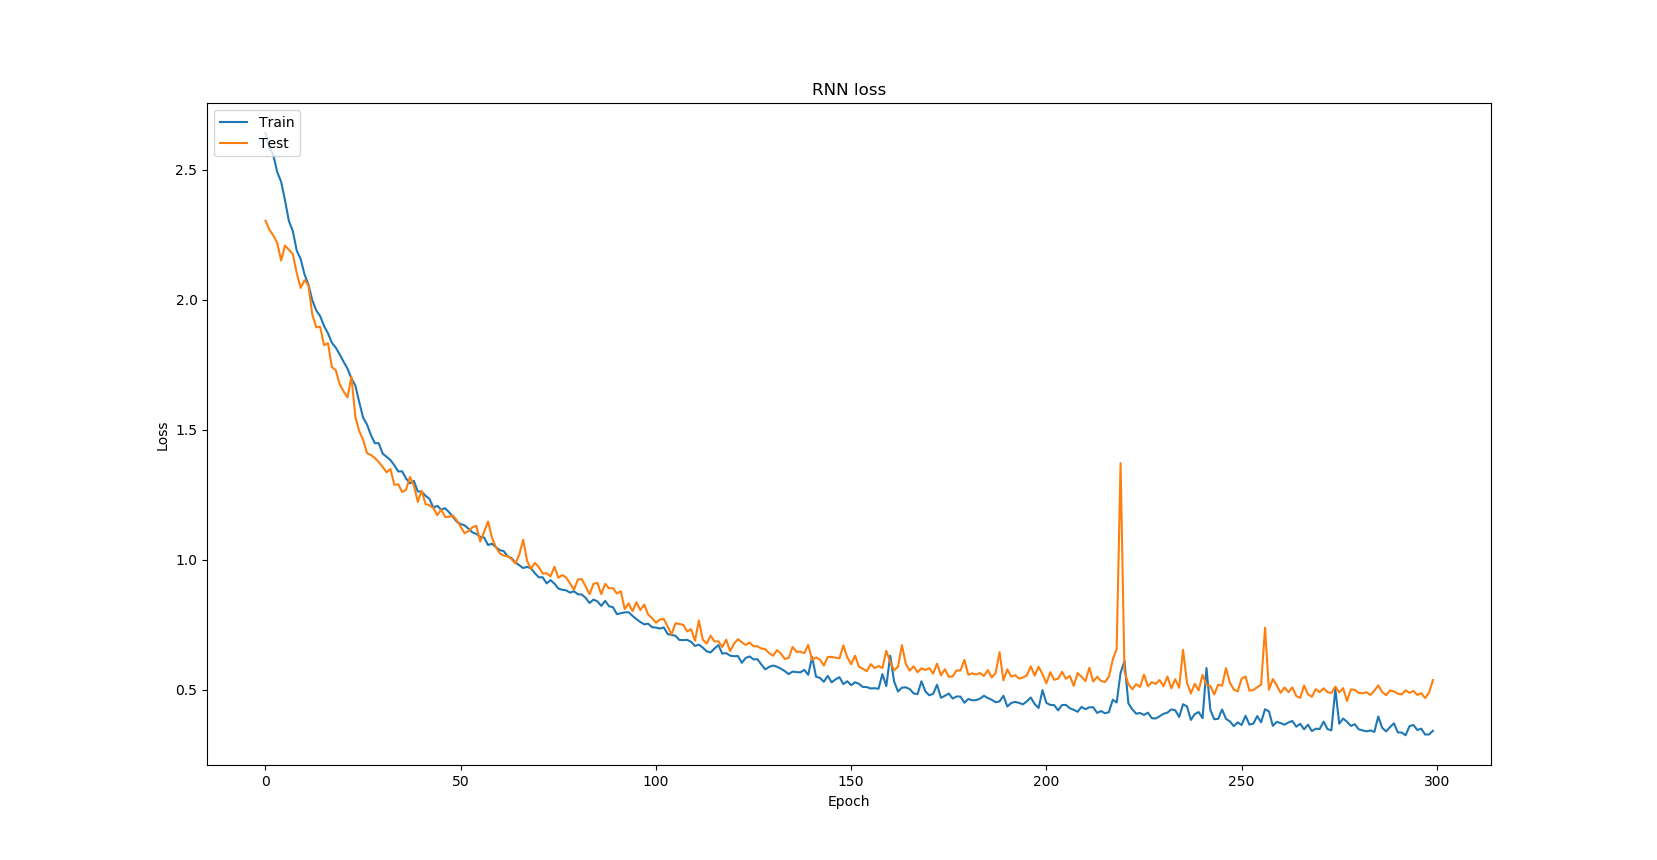
\includegraphics[scale=0.3]{300rnnl.png}
      \caption{Training and validation loss of RNN model.}
      \label{300rnnl}
    \end{figure}
  % \item LSTM:
    \begin{figure}[H]
      \centering
      \subfloat[LSTM's accuracy using SGD.]{{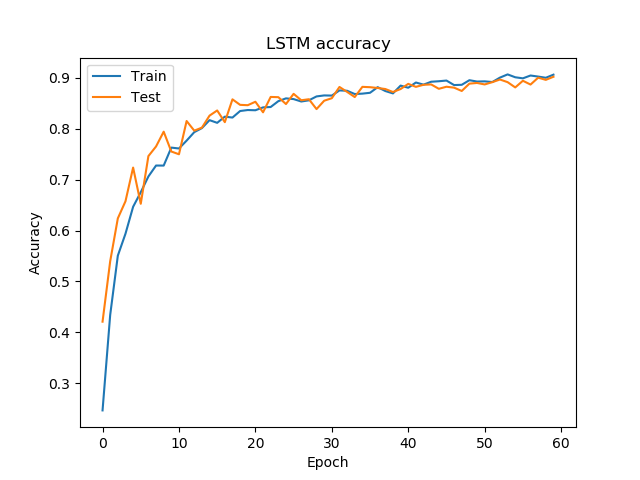
\includegraphics[scale=0.5]{sgdlstma.png} }}%
      \qquad
      \subfloat[LSTM's accuracy using Adam.]{{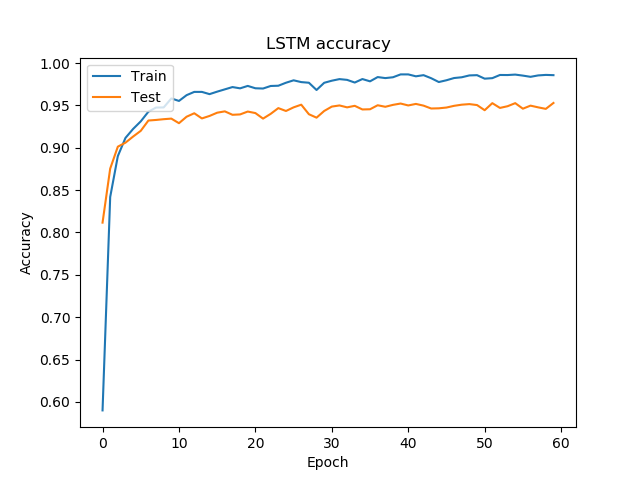
\includegraphics[scale=0.5]{adamlstma.png} }}%
      \caption{Accuracy comparison between LSTM using SGD and Adam.}%
      \label{lstma}
    \end{figure}
    \begin{figure}[H]
      \centering
      \subfloat[LSTM's loss using SGD.]{{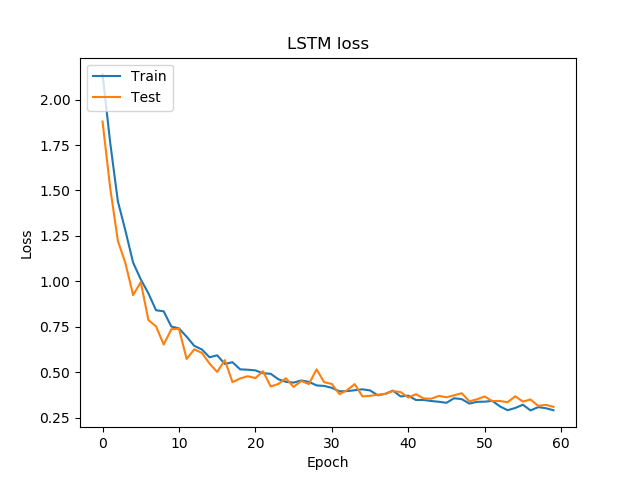
\includegraphics[scale=0.5]{sgdlstml.png} }}%
      \qquad
      \subfloat[LSTM's loss using Adam.]{{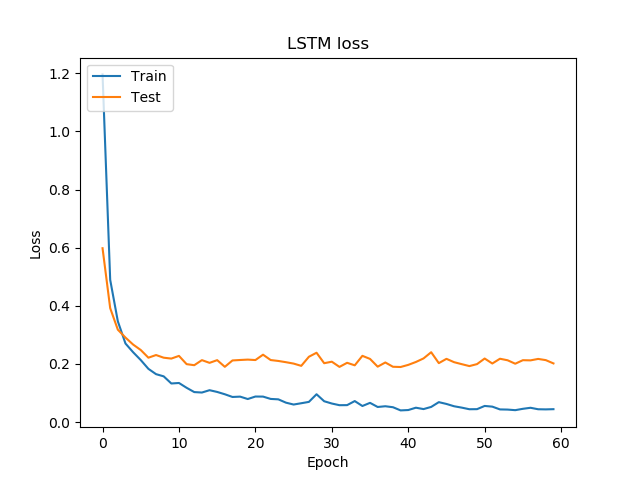
\includegraphics[scale=0.5]{adamlstml.png} }}%
      \caption{Loss comparison between LSTM using SGD and Adam.}%
      \label{lstml}
    \end{figure}
  % \item GRU:
    \begin{figure}[H]
      \centering
      \subfloat[GRU's accuracy using SGD.]{{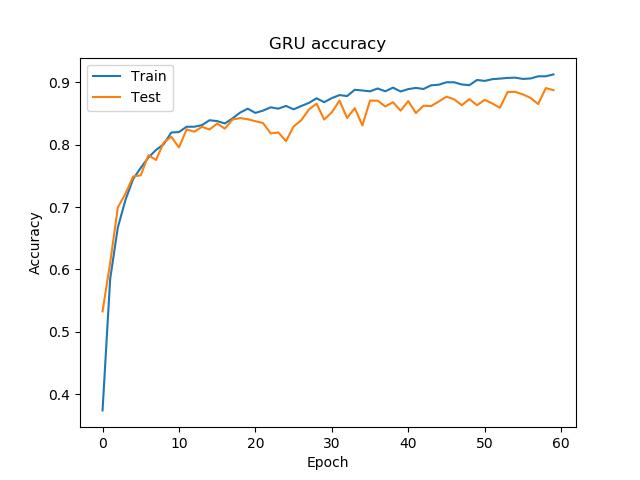
\includegraphics[scale=0.5]{sgdgrua.png} }}%
      \qquad
      \subfloat[GRU's accuracy using Adam.]{{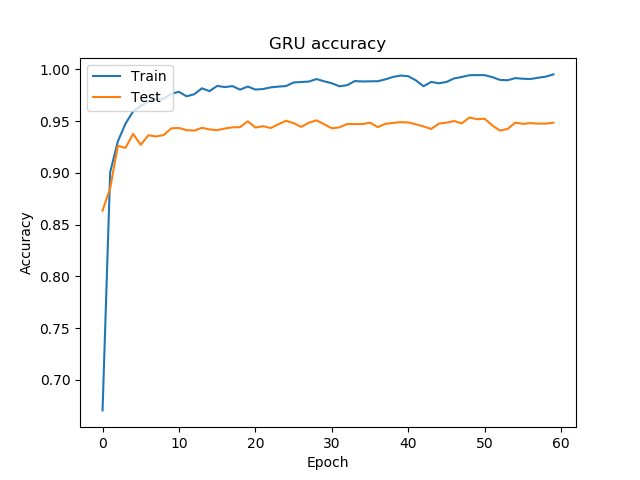
\includegraphics[scale=0.5]{adamgrua.png} }}%
      \caption{Accuracy comparison between GRU using SGD and Adam.}%
      \label{grua}
    \end{figure}
    \begin{figure}[H]
      \centering
      \subfloat[GRU's loss using SGD.]{{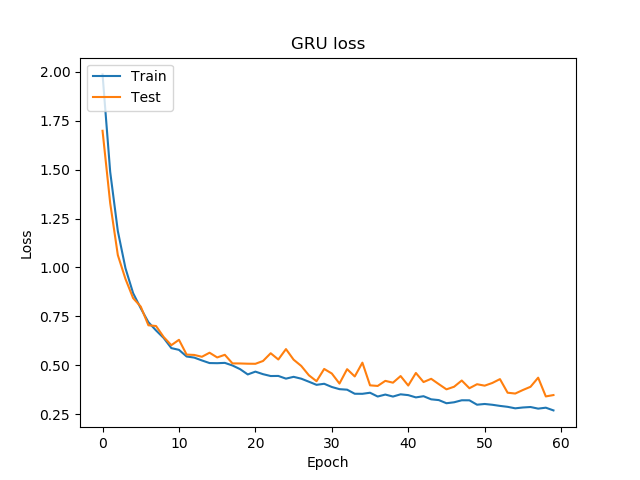
\includegraphics[scale=0.5]{sgdgrul.png} }}%
      \qquad
      \subfloat[GRU's loss using Adam.]{{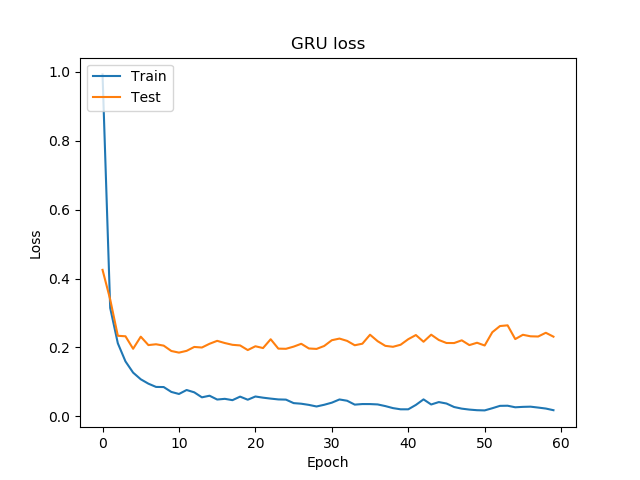
\includegraphics[scale=0.5]{adamgrul.png} }}%
      \caption{Loss comparison between GRU using SGD and Adam.}%
      \label{grul}
    \end{figure}
% \end{enumerate}

\textbf{Training on Luxembourghish dataset.}\\
\begin{figure}[h]
  \centering
  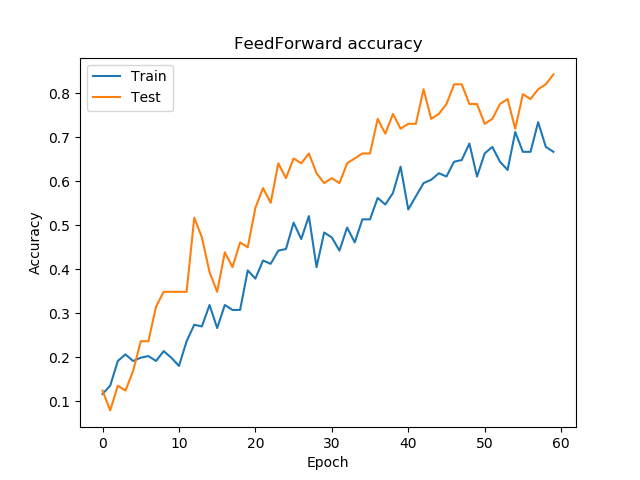
\includegraphics[scale=0.5]{luxffa.png}
  \caption{Training and validation accuracy of feedforward model trained on
  Luxembourgish dataset.}
  \label{luxffa}
\end{figure}

\begin{figure}[h]
  \centering
  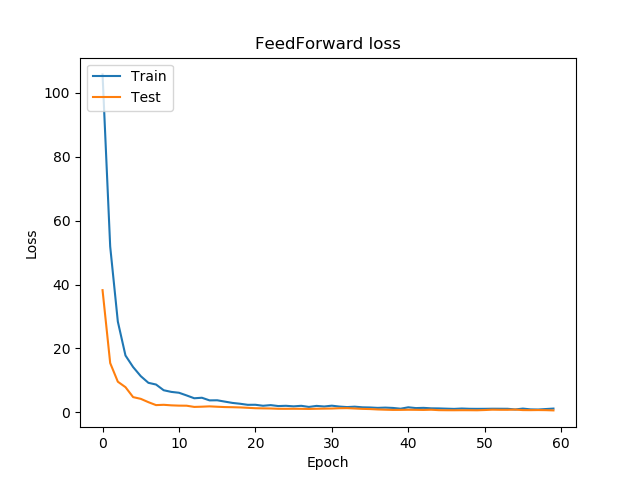
\includegraphics[scale=0.5]{luxffl.png}
  \caption{Training and validation loss of feedforward model trained on
  Luxembourgish dataset.}
  \label{luxffl}
\end{figure}

\begin{figure}[h]
  \centering
  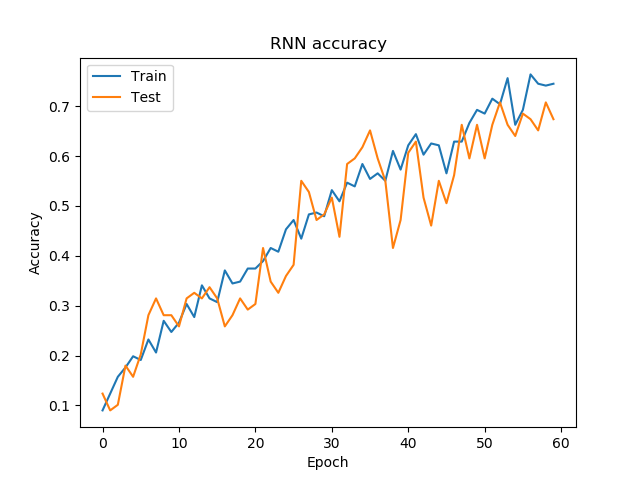
\includegraphics[scale=0.5]{luxrnna.png}
  \caption{Training and validation accuracy of RNN model trained on
  Luxembourgish dataset.}
  \label{luxrnna}
\end{figure}

\begin{figure}[h]
  \centering
  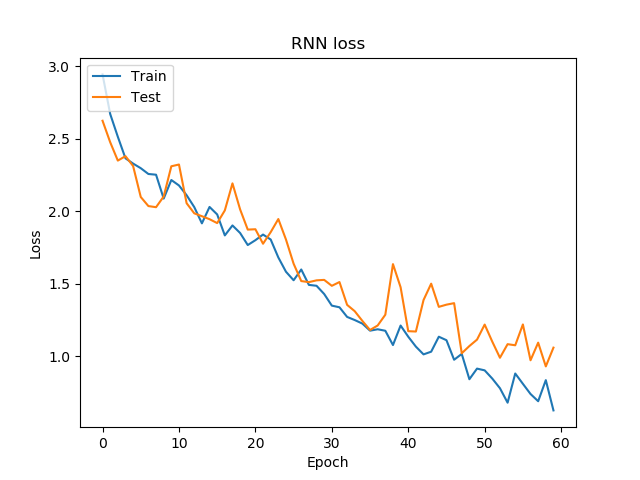
\includegraphics[scale=0.5]{luxrnnl.png}
  \caption{Training and validation loss of RNN model trained on Luxembourgish
  dataset.}
  \label{luxrnnl}
\end{figure}

\begin{figure}[h]
  \centering
  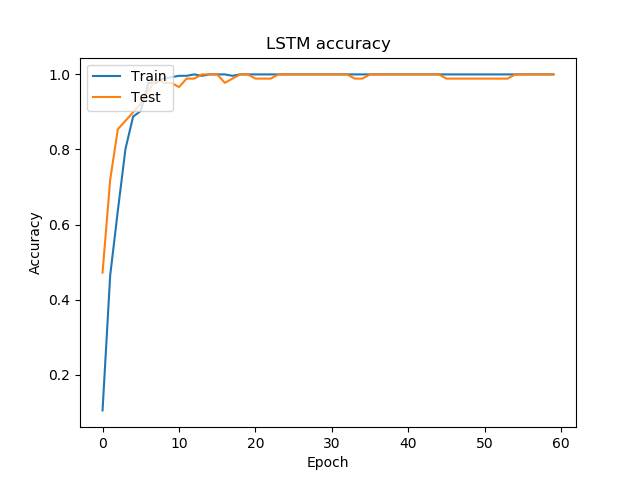
\includegraphics[scale=0.5]{luxlstma.png}
  \caption{Training and validation accuracy of LSTM model trained on
  Luxembourgish dataset.}
  \label{luxlstma}
\end{figure}

\begin{figure}[h]
  \centering
  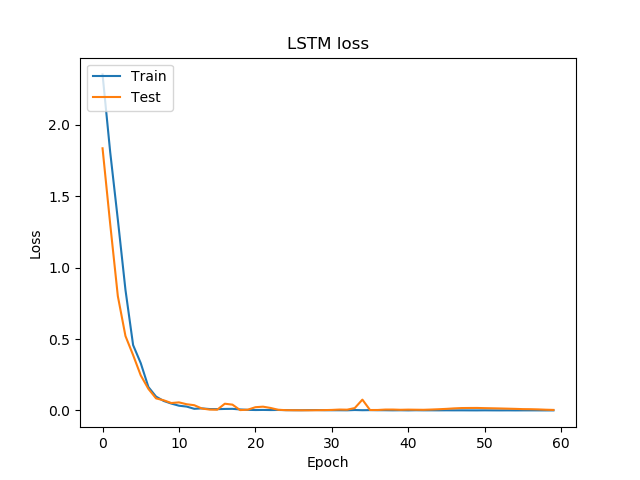
\includegraphics[scale=0.5]{luxlstml.png}
  \caption{Training and validation loss of LSTM model trained on Luxembourgish
  dadataset.}
  \label{luxlstml}
\end{figure}

\begin{figure}[h]
  \centering
  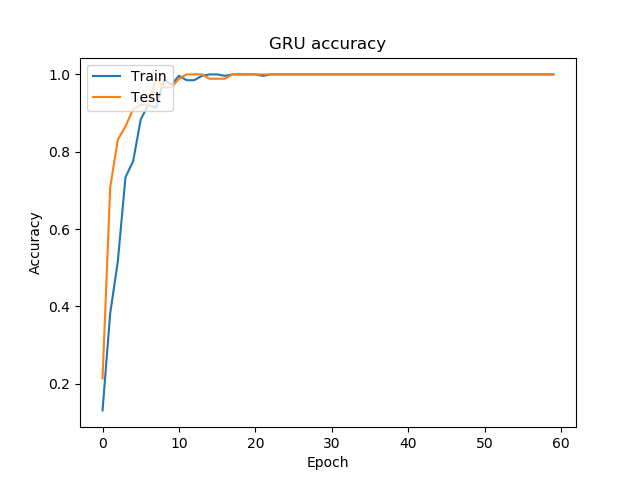
\includegraphics[scale=0.5]{luxgrua.png}
  \caption{Training and validation accuracy of GRU model trained on Luxembourgish
  dadataset.}
  \label{luxgrua}
\end{figure}

\begin{figure}[h]
  \centering
  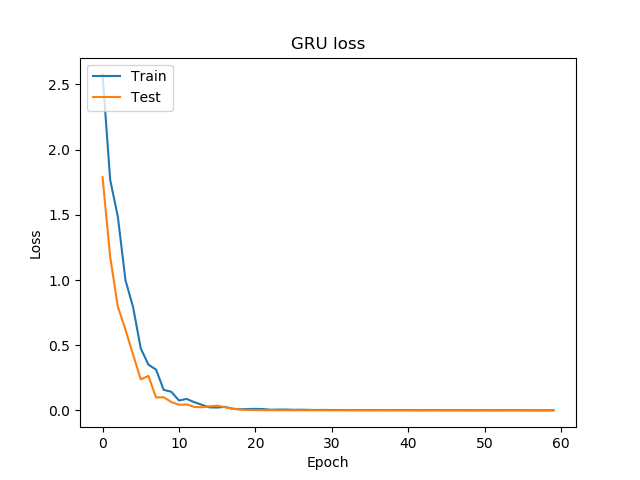
\includegraphics[scale=0.5]{luxgrul.png}
  \caption{Training and validation loss of GRU model trained on Luxembourgish
  dadataset.}
  \label{luxgrul}
\end{figure}

\begin{figure}[h]
  \centering
  \lstinputlisting{sections/scientific/fr1/mfccsnippet.py}
  \caption{Code snippet to extract MFCCs from the dataset.}
  \label{mfccsnip}
\end{figure}
